\chapter{Architectuur}\label{architectuur}
De oplossing die voorgesteld wordt in deze thesis is een monitoring library voor mobiele applicaties, Tracklytics genaamd. In deze sectie worden de architecturale beslissingen uitgelegd.\\

Tracklytics stelt een gehele infrastructuur voor die ontworpen werd om een mobiele applicatie te monitoren. In de volgende figuur \ref{fig:component} worden de belangrijkste componenten beschreven. De hoofdcomponenten zijn: \textit{TracklyticsCore, TracklyticsBackend en het Dashboard}. Deze vormen het aangeboden Tracklytics systeem. De \textit{UserApplication} stelt een mobiele applicatie voor die het Tracklytics systeem gebruikt. \\

Het Tracklytics systeem bestaat uit:
\begin{itemize}
\item een reusable/easy-to-use library voor mobiele applicaties (\textit{TracklyticsCore})
\item een back end service om de data uit de library te verwerken (\textit{TracklyticsBackend})
\item een dashboard dat de data uit de back end weergeeft aan de developer (\textit{Dashboard}).
\end{itemize}

Dit systeem kan gebruikt worden door mobiele applicaties om de applicatie te monitoren. De componenten van dit systeem zijn ontwikkeld om samen te werken en worden besproken in het volgende gedeelte van dit hoofdstuk. 


\begin{figure}[!h]
  \centering
  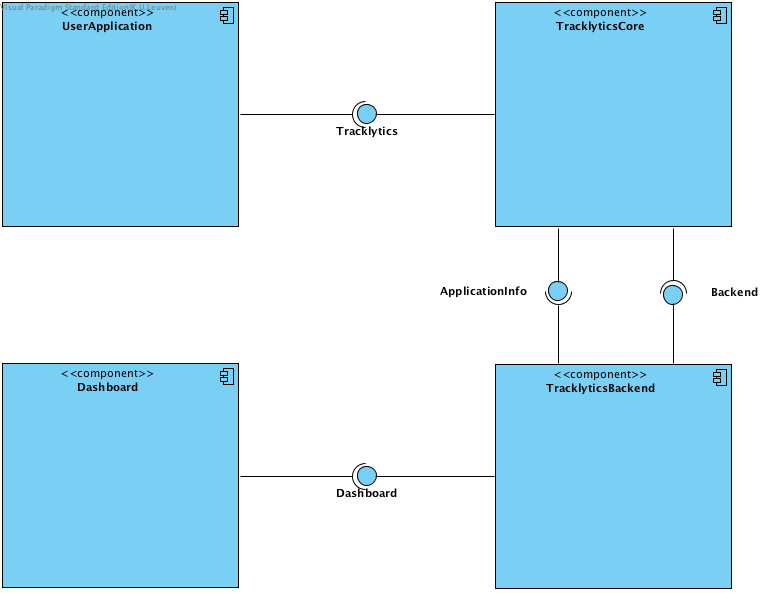
\includegraphics[scale=0.4]{Afbeeldingen/Architectuur/Component}
  \caption{Component diagram Tracklytics library.}
  \label{fig:component}
\end{figure}

\section{Component Diagram}
Het component diagram \ref{fig:component} duidt aan welke componenten een rol spelen in het bouwen van de Tracklytics library. In de volgende secties worden de verschillende componenten beschreven en hun rol wordt uitgelegd.


\subsection{UserApplication}
De UserApplication component representeert een applicatie ontwikkeld door developers. De UserApplication gebruikt de Tracklytics interface om metingen uit te voeren en de applicatie te monitoren. Om de developers te helpen bij het monitoren van de applicatie willen we mechanismen aanbieden om het design en de performance van de applicatie te monitoren. Om het design te monitoren willen we het monitoren van volgende elementen ondersteunen:
\begin{itemize}
\item op welke buttons/switches/entry in een tabel gebruikers drukken
\item welke schermen de gebruikers bezoeken
\item het gemiddeld aantal zoekresultaten per zoekopdracht
\item het gemiddelde of de verdeling van het getal dat een gebruiker in een bepaald veld invoert
\item hoe lang de applicatie gemiddeld gebruikt wordt
\end{itemize}

Om de performance van de applicatie op een hoog niveau te kunnen monitoren willen we volgende elementen kunnen monitoren:
\begin{itemize}
\item hoe lang een stuk code over het uitvoeren ervan doet om na te gaan of deze code niet te traag is.
\item de tijd die een request over het internet nodig heeft om te voltooien om te kijken of er hier een vertraging opgelopen wordt.
\item het gemiddeld aantal entries in een array of een NSDictionary (een Map in Java). Indien er ge\"itereerd wordt over deze datastructuren kan een groot aantal entries ervoor zorgen dat dat stuk code de applicatie vertraagt.
\item het gemiddeld aantal keer dat een bepaalde methode uitgevoerd wordt om te kijken

\end{itemize}


\subsection{TracklyticsCore}
De TracklyticsCore component vormt de belangrijkste component van de Tracklytics infrastructuur voor. Deze component bevat de monitoring library die ontwikkeld wordt in deze thesis. Deze component bevat de functionaliteit om de mobiele applicatie te monitoren. Voor elk soort element besproken in vorige sectie moet er een mechanisme ingebouwd zijn in deze component. \\

Om er zeker van te zijn dat alle data uiteindelijk in de back end geraakt via het netwerk, wordt er een optionele tijdelijke buffer/cache voorzien die de data tijdelijk naar de harde schijf van het toestel wegschrijft. Indien de data gesynchroniseerd is met de back end wordt deze data verwijderd van de harde schijf van het toestel. Dit mechanisme zorgt ervoor dat elke meting in de back end geraakt en er geen data verloren gaat. Het opslaan van deze data op de harde schijf vormt een extra indirectie.\\

In deze component bevindt zich een subcomponent die de communicatie met de back end verzorgt. Deze is verantwoordelijk voor het afleveren van de data van de metingen uit de library aan de back end. Het is de verantwoordelijkheid van deze subcomponent om alle meta-informatie over de applicatie op te halen uit te back end, zoals de voorkeuren die de developer heeft opgegeven in het dashboard. Deze subcomponent gebruikt een identifier voor de applicatie om deze correct te synchroniseren met de back end zodat het onderscheid kan gemaakt worden tussen deze applicatie en andere applicaties. 


\paragraph{Interface}
De TracklyticsCore component biedt een Tracklytics interface aan. De UserApplication kan deze interface gebruiken om de applicatie te monitoren. De TracklyticsCore stuurt deze data door naar de server.\\

De interface bestaat uit methodes om de applicatie te monitoren. Tracklytics biedt vijf elementen aan om de applicatie te kunnen monitoren, namelijk:
\begin{itemize}
\item \texttt{Counter}: kan gebruikt worden om evenementen te tellen
\item \texttt{Meter}: kan gebruikt worden om periodiek waardes op te halen.
\item \texttt{Histogram}: kan gebruikt worden om een waarde te verzamelen dat in het dashboard in een histogram gegoten kan worden. 
\item \texttt{Timer}: kan gebruikt worden om de lengte van een evenement te meten.
\item \texttt{Gauge}: kan gebruikt worden om een bepaalde waarde te meten. 
\end{itemize}

\subsection{Dashboard}
De Dashboard component representeert een applicatie om de gemonitorde data van de Tracklytics library weer te kunnen geven aan de developers en de eigenaars. Met behulp van grafieken en verwerkte data kunnen de developers en de eigenaars beslissingen nemen omtrent de applicatie. In dit dashboard kunnen instellingen aangegeven worden door de developer voor de applicatie. \\

\subsection{TracklyticsBackend}
De TracklyticsBackend component representeert de server kant van de library. Hierop draait de code om de gemonitorde data op te slaan in de database. De TracklyticsBackend component bevat dus de database om alle informatie in op te slaan. \\
De TracklyticsBackend component biedt drie interfaces aan, namelijk: ApplicationInfo, Backend en Dashboard. Deze worden in de volgende sectie besproken.\\

De TracklyticsBackend behandelt elke request die binnenkomt van het Dashboard of van de TracklyticsCore. Om de request van de TracklyticsCore te beantwoorden voegt hij alle informatie die in de request staat toe aan de database en zendt hij een bericht terug met de boodschap dat de request succesvol afgerond werd of een boodschap met een foutmelding in, zodat de TracklyticsCore deze fout kan verwerken. Om een request van het Dashboard af te werken haalt de TracklyticsBackend de gewenste gegevens uit de database, verwerkt deze informatie en geeft de verwerkte informatie door aan de back end om weer te geven. Om deze functionaliteit aan te bieden moet de TracklyticsBackend een connectie hebben met de database. 



\subsubsection{Interfaces}
\paragraph{ApplicationInfo}
Deze interface wordt gebruikt door de TracklyticsCore component om voorkeuren die de developer heeft gemaakt in het dashboard op te halen en toe te passen op de monitoring library.

\paragraph{Backend}
Deze interface wordt gebruikt om data uit te wisselen tussen de TracklyticsCore en de TracklyticsBackend. Dit is de gemonitorde data die de TracklyticsCore verzameld heeft. De TracklyticsBackend verwerkt deze informatie en slaat deze op in de database.\\

\paragraph{Dashboard}
Deze interface wordt gebruikt door het dashboard om de data uit de database op te halen om deze weer te kunnen geven aan de developers. 





\begin{figure}[!h]
  \centering
  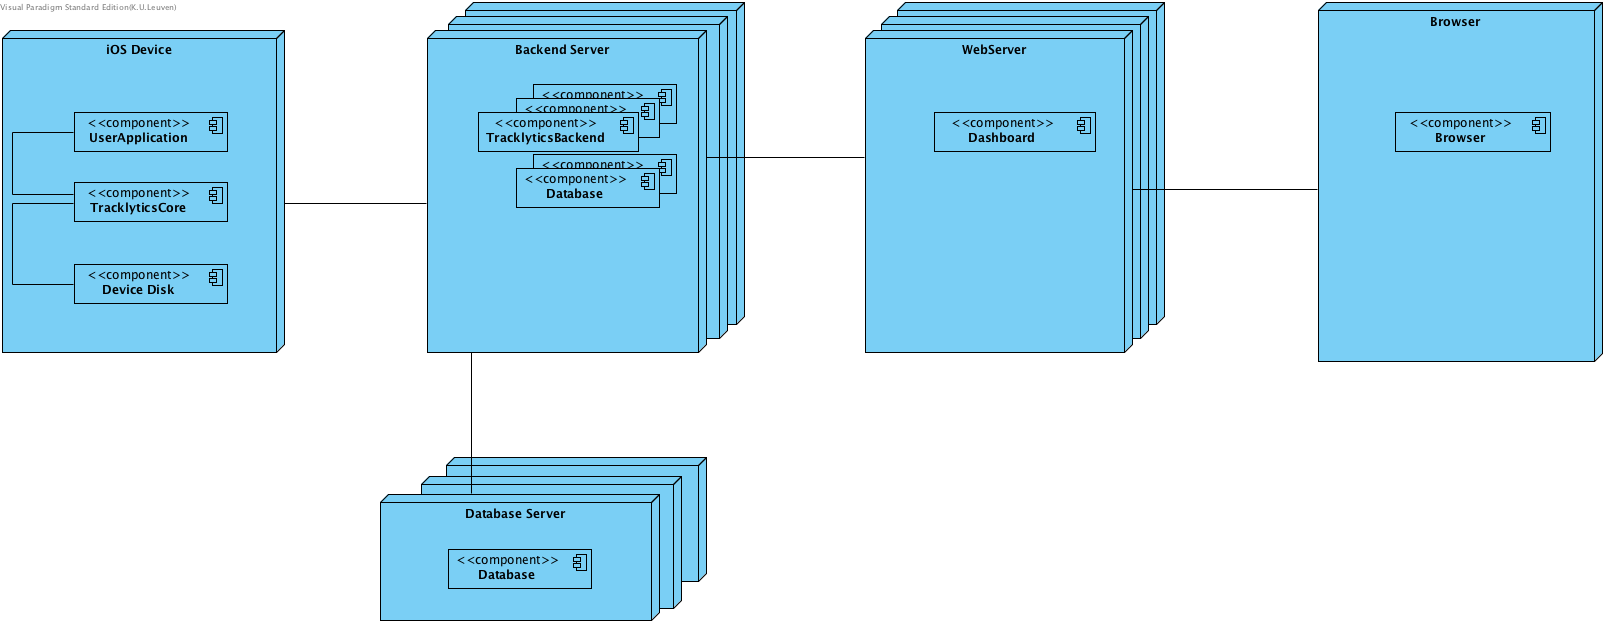
\includegraphics[scale=0.30]{Afbeeldingen/Architectuur/Deployment}
  \caption{Deployment diagram Tracklytics library.}
  \label{fig:deployment}
\end{figure}
\section{Deployment Diagram}
Het deployment diagram toont op welke nodes de componenten, besproken in vorige sectie, draaien. Zoals je kan zien draait de UserApplication en de TracklyticsCore op het mobiele toestel van de gebruiker zelf. De TracklyticsBackend draait op een backend server die gerepliceerd kan worden. Deze staat in verbinding met een Database server waar alle data wordt opgeslagen. Het Dashboard draait op een webserver. Deze staat in verbinding met de backend server om de data te kunnen ophalen.

\section{Belangrijkste flows}
In deze sectie worden de belangrijkste flows in de Tracklytics library beschreven. Deze geven aan hoe de data flow binnen Tracklytics werkt.\\
De belangrijkste flows door Tracklytics zijn:
\begin{itemize}
\item tracking en monitoring van gegevens
\item verzenden en opslaan van de gegevens
\end{itemize} 


\subsection{Tracking en monitoring van gegevens}\label{sec:TrackingEnMonitoringVanGegevens}
\begin{figure}[!h]
  \centering
  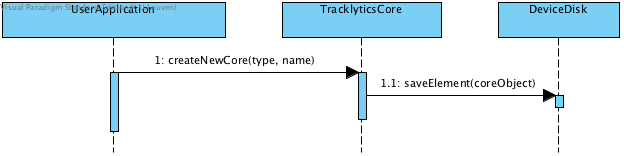
\includegraphics[scale=0.4]{Afbeeldingen/Architectuur/FlowDiagram1}
  \caption{Aanmaken van een core object van de Tracklytics library.}
  \label{fig:flow1}
\end{figure}
\begin{figure}[!h]
  \centering
  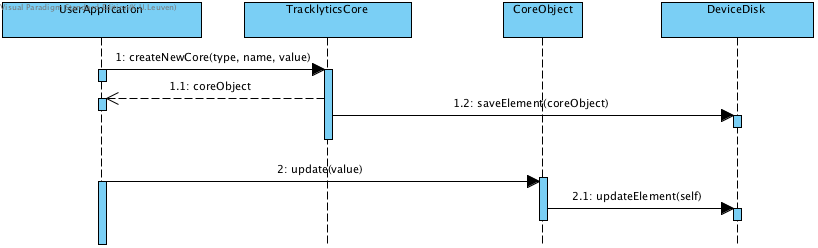
\includegraphics[scale=0.4]{Afbeeldingen/Architectuur/FlowDiagram2}
  \caption{Aanmaken en aanpassen van een core object van de Tracklytics library via de update call.}
  \label{fig:flow2}
\end{figure}

Het monitoren van de gegevens van de applicatie kan opgesplitst worden in twee verschillende flows. \\

De eerste flow \ref{fig:flow1} toont de meest simpele flow. De developer geeft aan dat een bepaalde waarde gecollecteerd moet worden. De TracklyticsCore houdt deze waarde in de cache totdat deze gesynchroniseerd wordt naar de server, wat getoond wordt in \ref{sec:VerzendenEnOpslaanVanGegevens}. Indien de developer dit aangegeven heeft, slaat de TracklyticsCore deze waarde op de harde schijf van het toestel op totdat deze waarde gesynchroniseerd wordt met de back end. Deze situatie is geldig wanneer er geen object wordt teruggegeven aan de developer om hierop functies te kunnen aanroepen. \\

De tweede flow \ref{fig:flow2} toont een uitbreiding op de eerste flow \ref{fig:flow1}. In deze situatie geeft de TracklyticsCore een object terug aan de developer. Op dit object kan de developer verschillende functies uitvoeren om de data te manipuleren via een update call. De TracklyticsCore past deze update toe op de gecachete waarde en de kopie die op de harde schijf van het toestel staat, indien deze bestaat. In plaats van dat een object uit de cache of van de harde schijf verwijderd wordt, houdt de TracklyticsCore deze bij tot de applicatie wordt afgesloten. Bij het heropstarten van de applicatie moeten deze objecten gesynchroniseerd worden met de server en verwijderd worden van de harde schijf. De objecten zijn al verwijderd uit de cache door het afsluiten van de applicatie.


\subsection{Verzenden en opslaan van de gegevens} \label{sec:VerzendenEnOpslaanVanGegevens}
In het volgende diagram \ref{fig:flow3} wordt getoond hoe het verzenden van de gegevens van het toestel naar de server in zijn werk gaat en hoe de gegevens worden opgeslagen in de database. \\
\begin{figure}[!h]
  \centering
  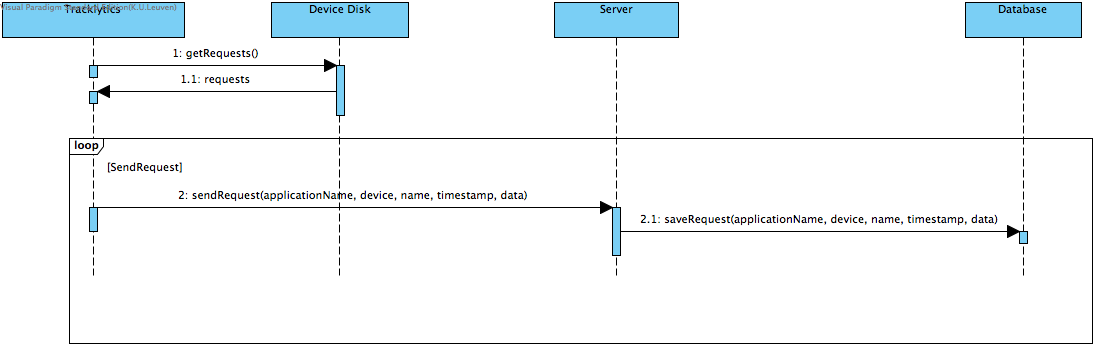
\includegraphics[scale=0.4]{Afbeeldingen/Architectuur/FlowDiagram3}
  \caption{Gegevens verzenden vanuit de library naar de back end}
  \label{fig:flow3}
\end{figure}

Om de data naar de TracklyticsBackend te verzenden, haalt de TracklyticsCore de gegevens die op de harde schijf staan op en voegt deze samen met de gegevens die in zijn cache staan. De TracklyticsCore itereert over deze samengevoegde gegevens en verzend deze naar de server. De server verwerkt de data die doorgestuurd werd en slaat deze verwerkte data op in de database. De server stuurt een antwoord terug naar de TracklyticsCore met daarin ofwel een succes boodschap en een identifier van het object in de database, ofwel met een error message. De TracklyticsCore verwerkt deze boodschap: ofwel is het object een object van het type dat beschreven werd in \ref{fig:flow1}, dan verwijdert de component het object uit zijn cache en van de harde schijf van het toestel. Ofwel is het een object van het type beschreven in \ref{fig:flow2}, dan moet hij de identifier dat mee werd gestuurd in het bericht toewijzen aan dat object, zodat bij een update het object wordt aangepast in de database in plaats van dat er een tweede object in de database geplaatst wordt. Ofwel is het een error message, dan moet de TracklyticsCore ofwel opnieuw proberen te synchroniseren, ofwel wachten tot de volgende synchronisatie om het object naar de server door te sturen.\\

\section{Uitbreidingen}
In deze sectie worden een aantal uitbreidingen besproken die niet standaard in een monitoring library zitten, maar zeer handig kunnen zijn om developers te helpen bij het monitoren van de applicatie.

\paragraph{Data availability}
Smartphones vallen weleens zonder internet connectiviteit door het wegvallen van een WiFi verbinding of het wegvallen van de mobiele verbinding. De Tracklytics library zendt de gemonitorde data over het internet naar de back end om deze op te slaan in een database. Als de internetverbinding zou wegvallen, dan zou er mogelijks belangrijke data verloren gaan. Om dit scenario te voorkomen slaan we de data tijdelijk op op de harde schijf van de mobiele telefoon. Indien de smartphone dan terug verbinding met het internet heeft gemaakt kan de data alsnog gesynchroniseerd worden met de back end. De data wordt tijdelijk opgeslagen, dus nadat de data gesynchroniseerd is, wordt deze van de smartphone verwijderd. Zo wordt ervoor gezorgd dat de data in ieder geval in de database terecht komt. 

\paragraph{On Demand}\label{par:OnDemand}
Het is de bedoeling de developer zoveel mogelijk vrijheid te geven in het monitoren van de applicatie. Om deze vrijheid te verhogen werd het On Demand aan- of uitzetten van het monitoren aan Tracklytics toegevoegd. Een developer kan vanuit het dashboard aangeven of de applicatie op dit moment gemonitord moet worden of niet. Dit kan gebruikt worden om op de piekdagen of piekmomenten het monitoren aan te zetten. Zo kan uitgezocht worden of er een bottleneck bestaat als het gebruik van de applicatie piekt. \\
Indien een developer ontdekt dat er geen bottleneck of problemen zijn met de app en deze niet verder gemonitord moet worden, dan is het handig om de monitoring uit te kunnen zetten. Het uitzetten van het monitoren zorgt ervoor dat de prestatiekost van de library ge\"elemineerd wordt in de applicatie.


\paragraph{Aggregatie}\label{Arch:Aggregatie}
De data die doorgestuurd wordt naar de server heeft enkel betrekking op de specifieke gebruiker van de applicatie op zijn telefoon. Om een overzicht te geven van wat de algemene trend is van deze metingen, is het nodig deze data samen te voegen met de data van alle andere gebruikers en deze te aggregeren om een goede analyse hiervan te maken. Er zijn twee plaatsen waar deze aggregatie uitgevoerd kan worden, namelijk op de smartphone zelf in de Tracklytics library of in de back end. \\

Om bandbreedte te besparen en om verwerkingstijd in de back end te besparen is er de mogelijkheid om de data op het toestel van de gebruiker te aggregeren. Enkel de geaggregeerde data wordt doorgestuurd naar de back end die deze dan in geaggregeerde vorm in de database opslaat. Indien het dashboard deze data dan opvraagt, moet de back end deze data nog samenvoegen, wat minder tijd en bandbreedte vraagt van de database, omdat de data kleiner is. De back end kan deze data sneller verwerken, omdat hij enkel de geaggregeerde data moet verwerken en niet alle data die de library heeft vergaard. Het nadeel hieraan is dat sommige statistieken (zoals bijvoorbeeld de mediaan) een benadering van de werkelijke mediaan wordt. \\

De reden om de aggregatie op de back end uit te voeren is dat de back end een grotere verwerkingskracht heeft dan het toestel van de gebruiker en de back end heeft als enige taak data te verwerken en op te slaan in de database en data uit de database te halen, terwijl het toestel naast het monitoren van de applicatie de taak heeft om de applicatie uit te voeren. De back end moet in deze situatie alle data ophalen en verwerken, wat veel bandbreedte en verwerkingskracht kost indien het totaal aantal meetpunten groot is. \\

Een derde mogelijkheid is om de gebruikers op te delen in twee verschillende groepen, waarbij de ene groep de data aggregeert op het toestel en de andere de aggregatie laat doen in de back end. De back end moet de geaggregeerde en de niet-geaggregeerde data samenbrengen en verwerken indien het dashboard deze opvraagt. Een typische eigenschap is om de groep op te delen op type toestel. Zo kunnen toestellen met een tragere CPU de aggregatie laten gebeuren in de back end en de toestellen met een snellere CPU de aggregatie uitvoeren op het toestel zelf. \\

Een andere mogelijkheid is om een deel van de data te aggregeren op het toestel en een deel van de data in de back end te laten aggregeren. Zo wordt er toch bandbreedte bespaard en wordt de benadering van bijvoorbeeld de mediaan juister dan dat alles op het toestel van de gebruiker geaggregeerd wordt. De developer moet de mogelijkheid gegeven worden om het percentage van de data dat geaggregeerd moet worden op het toestel aan te geven. Zo kan de developer het percentage zoeken dat het best bij zijn applicatie past.\\ 

Een functie in het dashboard zou ervoor kunnen zorgen dat de developer de optie krijgt om \'e\'en van deze mogelijkheden te kiezen die op dit moment actief zou moeten zijn. Zo wordt de developer de vrijheid gegeven om de library te tweaken naar zijn voorkeuren.

\paragraph{AB Testing}
AB testing kan gezien worden als een mechanisme dat grote bedrijven, zoals facebook, gebruiken om nieuwe features uit te rollen naar de gebruikers. Het mechanisme werkt als volgt: er bestaat een versie A en een versie B van de software met B de nieuwere versie. AB testing zorgt ervoor dat de uitrol van versie B geleidelijk verloopt. De gebruikers van de software worden dus in twee (of meerdere) groepen opgedeeld door een bepaalde eigenschap. Deze eigenschap kan eender welke vorm aannemen, bijvoorbeeld: geografische locatie, ingestelde taal, de gebruikte browser, het type toestel, enz. Indien er zich dan een probleem voordoet in versie B, dan bestaat dit enkel bij de groep die versie B al verkregen heeft en dus niet bij alle gebruikers. Hierdoor merkt enkel die groep dat er een probleem bestaat en kan versie B aangepast worden om dit probleem op te lossen of eventueel kan ervoor gezorgd worden dat iedereen terug versie A gebruikt tot het probleem in versie B opgelost wordt. \\

In mobiele applicaties is het moeilijker om echt aan AB testing te doen, omdat deze applicaties meestal statisch zijn. Er moet een update in de app store komen om een nieuwe versie met nieuwe features en code uit te rollen. Dit staat pal tegenover websites die hun webpagina's en code rechtstreeks van een server halen en waar de aanpassingen aan de versies meteen zichtbaar zijn bij de gebruikers. 
Een workaround van dit probleem is dat de mobiele applicatie de code van de nieuwe versie (B) al kan bevatten en ook nog de code van de oude versie (A) erin heeft staan. Tracklytics kan dan een functie in het dashboard aanbieden om de groepen op te delen in twee (of meerdere) groepen op basis van eigenschappen die de developer kan kiezen. In de mobiele applicatie moeten we dus dat onderscheid kunnen maken welke code aangeroepen moet worden. De gemakkelijkste oplossing is om een codenaam aan de versie toe te voegen, zodat er meerdere versies van de code aanwezig kan zijn. 
Het nadeel van dit mechanisme is dat de applicatie groter is dan hij zou zijn, moest de applicatie enkel de code bevatten die voor die bepaalde groep nodig is.


\paragraph{Security \& Privacy}
De privacy van de gebruiker wordt gezien als een belangrijk aspect. Zoals eerder al aangehaald, is NewRelic een closed source library, wat wil zeggen dat developers niet weten welke informatie er doorgestuurd wordt naar de back end. Dit gegeven zorgt ervoor dat privacygevoelige applicaties deze library niet zouden mogen gebruiken, omdat er gebruikersinformatie gelekt zou kunnen worden naar de back end van NewRelic zoals bijvoorbeeld email-adressen, creditcard gegevens, etc.\\
Deze reden heeft ervoor gezorgd dat ervoor gekozen werd om de Tracklytics library open source te maken. Zo kunnen developers zeker zijn welke informatie er wordt doorgestuurd naar de back end en wordt de privacy van de gebruiker wel gegarandeerd. Tracklytics verzamelt enkel metadata van de telefoon en de applicatie. De metadata die gecollecteerd wordt door Tracklytics bestaat uit: het type toestel, de versie, de naam van de applicatie, een identifier van de applicatie, een identifier van het toestel om deze van elkaar te kunnen onderscheiden, de datum en het type connectie waarop het toestel zich bevindt. Dit gegeven zorgt ervoor dat Tracklytics de privacy van de gebruiker garandeert..\\

Naast privacy vormt security ook een belangrijk aspect. Er bestaat namelijk een verbinding tussen de mobiele applicatie en de back end over een onveilig netwerk. Het zou dus niet mogen dat de doorgezonden data door een onrechtmatig iemand gecollecteerd wordt of dat hiermee geknoeid wordt. Om deze situaties te voorkomen werd ervoor gekozen om via een HTTPS verbinding te werken. Deze verbinding zorgt uit zichzelf voor een veilige verbinding tussen begin- en eindpunt. Als extra veiligheid werkt Tracklytics met HTTP Post in plaats van HTTP Get, zodat de doorgegeven data niet zichtbaar wordt in de URL naar de back end. Deze combinatie zorgt ervoor dat de gegevens niet onderschept kunnen worden door onrechtmatige personen. 




%%% Local Variables: 
%%% mode: latex
%%% TeX-master: "masterproef"
%%% End: 
